\section{My Solutions to the Problem}

	The car gets binary inputs ($\ket{0}$ and $\ket{1}$) from two sensors attached to it. We need to build a quantum circuit to give the output to the motors like the \hyperref[table:1]{\textit{Table 1}}.
	
	In the ~\cite{mahanti2019quantum} article, the authors tried to solve the problem by defining a new sort of quantum gate, the \textbf{two-control-two-target Toffoli (C\textsubscript{2}(X\textsuperscript{3}X\textsuperscript{4})) gate}. They also made a large Quantum Circuit. But, I found some much easier and smaller approaches to the problem.	
	\vspace{3mm}

	\noindent {\large From the \hyperref[table:1]{\textit{Table 1}}, we can say that:}
	
	\begin{itemize}
		\item M1 = not(S2) = $\sim$ S2
		\item M2 = not(S1) = $\sim$ S1
		\item M3 = S1 and S2 = S1 $\land$ S2
	\end{itemize}
	\noindent {\large I came up with two easier solutions:}
	\begin{enumerate}
		\item \textbf{5 cubit:} This approach uses 5 qubits. We use two Quantum Registers for the sensor inputs, and the rest three for the motor outputs.
		\item \textbf{3 cubit:} This approach uses 3 qubits. Here, we have two Quantum Registers for taking input from the two sensors. We process those signals and use them as inputs to the first two motor. We use the third Quantum Registers for output to the third motor.
	\end{enumerate}

	\subsection{Approach 1: 5 Cubit Solution}
	\label{solution:1}
		\subsubsection{Importing the libraries}
\label{code:importing_the_libraries}
\begin{lstlisting}[language=Python]
from qiskit import *
from qiskit.visualization import *\end{lstlisting}

\subsubsection{Making the Quantum Circuit}
\textbf{Making the Qiskit Classes:}
\label{code:making_the_qiskit_classes}
\begin{lstlisting}[language=Python]
# 1. making the sensor registers
sensors = QuantumRegister(2, 'sensor')
# 2. making the motor registers
motors = QuantumRegister(3, 'motor')
# 3. making the classical registers, 1 for each motors
creg_c = ClassicalRegister(3, 'measurements')
# 4. Adding the registers to get the quantum circuit
circuit = QuantumCircuit(sensors, motors, creg_c)\end{lstlisting}
\vspace{3mm}

\textbf{Initializing the Circuit:} Demonstrating initialization with sensor value as = $\ket{10}$. Please feel free to try out the other states ($\ket{00}$, $\ket{01}$ and $\ket{11}$). This is Similar to the digitalRead function of Arduino.
\label{code:initializing_the_circuit}
\begin{lstlisting}[language=Python]
ket_0 = [1, 0]
ket_1 = [0, 1]

# quantumRead = [ket_0, ket_0] # |00>
# quantumRead = [ket_0, ket_1] # |01>
quantumRead = [ket_1, ket_0]   # |10>
# quantumRead = [ket_1, ket_1] # |11>

circuit.initialize(quantumRead[0], [sensors[0]])
circuit.initialize(quantumRead[1], [sensors[1]])\end{lstlisting}
\vspace{3mm}

\textbf{Designing the circuit:}
\label{code:designing_the_circuit}
\begin{lstlisting}[language=Python]
circuit.ccx(sensors[0], sensors[1], motors[2])
circuit.x(sensors[0])
circuit.x(sensors[1])
circuit.cx(sensors[0], motors[1])
circuit.cx(sensors[1], motors[0])
circuit.barrier()
circuit.measure(motors[0], creg_c[2])
circuit.measure(motors[1], creg_c[1])
circuit.measure(motors[2], creg_c[0])
circuit.draw(output = 'mpl')\end{lstlisting}

\begin{figure}[h]%
	\centering
	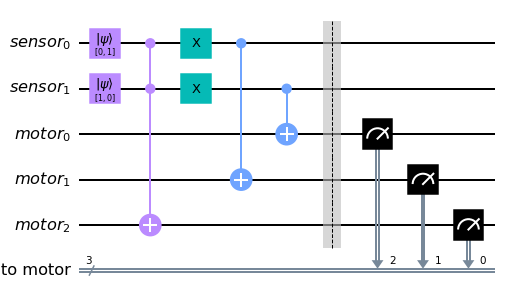
\includegraphics[width=0.9\linewidth]{./images/5qubit_qc.png}
	\caption{Circuit of the 5 Qubit Design}%
	\label{fig:5qubit_qc}%
\end{figure}

\subsubsection{Executing the Quantum Circuit on a Simulator}
\label{code:executing_the_quantum_circuit_on_a_simulator}
\begin{lstlisting}[language=Python]
comp = Aer.get_backend("qasm_simulator")
results = execute(circuit, comp, shots = 1024).result()
print("results:", results.get_counts(circuit))
plot_histogram(results.get_counts(circuit))\end{lstlisting}

{\fontfamily{pcr}\selectfont \noindent results: \{`100': 1024\}}
\vspace{5mm}

We got the result $\ket{100}$ with 100\% probability as output from the circuit after giving $\ket{10}$ as input. This matches with the \hyperref[table:1]{\textit{Table 1}}. We also checked the other 3 input cases ($\ket{00}$, $\ket{01}$ and $\ket{11}$) and verified that the circuit is working as expected.

\textbf{Note:} The probability came out to be 100\%, which is an ideal result. But in real world situations there is always some error involved in the measurement. The probability of getting the other results is not zero in those cases.

\begin{figure}[h]%
	\centering
	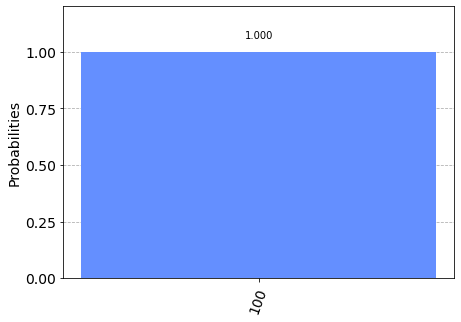
\includegraphics[width=0.7\linewidth]{./images/5qubit_sim.png}
	\caption{\textbf{Histogram:} 5 Qubit circuit executed on a simulator}%
	\label{fig:5qubit_sim}%
\end{figure}


\subsubsection{Executing the Quantum Circuit on an actual Quantum Computer}
\label{code:executing_the_quantum_circuit_on_a_quantum_computer}
\textbf{Importing the relevant libraries}
\label{code:importing_the_libraries_2}
\begin{lstlisting}[language=Python]
from qiskit.providers.ibmq import least_busy
from qiskit.tools.monitor import job_monitor
from qiskit.providers.ibmq.ibmqbackend import IBMQSimulator
# IBMQ.load_account(<API_Token>)
IBMQ.load_account()\end{lstlisting}
{\fontfamily{pcr}\selectfont <AccountProvider for IBMQ(hub='ibm-q', group='open',\par
project='main')>}
\vspace{3mm}

\textbf{Choosing the least busy backend}

\begin{lstlisting}[language=Python]
provider = IBMQ.get_provider('ibm-q')
q_comp = least_busy(
	[x for x in provider.backends() if not isinstance(x, IBMQSimulator)]
	)\end{lstlisting}
\vspace{3mm}

\textbf{Executing the circuit on a Quantum Computer}

\begin{lstlisting}[language=Python]
job = execute(circuit, q_comp, shots = 16384)
job_monitor(job)
print("results:", job.result().get_counts(circuit))
plot_histogram(job.result().get_counts(circuit))\end{lstlisting}

{\fontfamily{pcr}\selectfont
\noindent Job Status: job has successfully run

\noindent results:\par
\{`000': 819,\par
`001': 438,\par
`010': 157,\par
`011': 112,\par
`100': 12416,\par
`101': 1399,\par
`110': 877,\par
`111': 166\}}

\begin{figure}[h]%
	\centering
	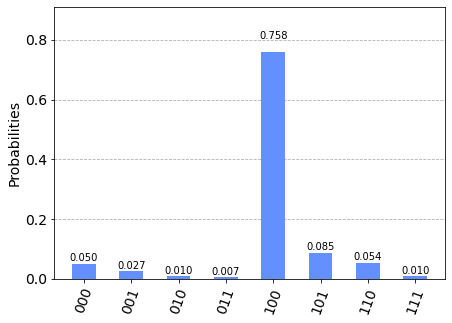
\includegraphics[width=0.9\linewidth]{./images/5qubit_act.png}
	\caption{\textbf{Histogram:} 5 Qubit circuit executed on an actual Quantum Computer}%
	\label{fig:5qubit_act}%
\end{figure}

	\subsection{Approach 2: 3 Cubit Solution}
	\label{solution:2}
		\textbf{Importing the libraries:}
This part is the same as \hyperref[code:importing_the_libraries]{`Importing the libraries'} section from the \hyperref[solution:1]{Approach 1}.

\textbf{Making the Quantum Circuit:}
\begin{lstlisting}[language=Python]
# Making the Qiskit Classes:
qreg_s1_to_m2 = QuantumRegister(1, 's1_to_m2')
qreg_s2_to_m1 = QuantumRegister(1, 's2_to_m1')
qreg_to_m3 = QuantumRegister(1, 'to_m3')
creg_measurements = ClassicalRegister(3, 'measurements')
circuit = QuantumCircuit(
	qreg_s1_to_m2,
	qreg_s2_to_m1,
	qreg_to_m3,
	creg_measurements
	)

# Initializing the Circuit:
ket_0 = [1, 0]
ket_1 = [0, 1]
quantumRead = [ket_1, ket_0]   # |10>
circuit.initialize(quantumRead[0], [qreg_s1_to_m2[0]])
circuit.initialize(quantumRead[1], [qreg_s2_to_m1[0]])

# Designing the circuit
circuit.ccx(qreg_s1_to_m2[0],qreg_s2_to_m1[0],qreg_to_m3[0])
circuit.x(qreg_s1_to_m2[0])
circuit.x(qreg_s2_to_m1[0])
circuit.barrier()
circuit.measure(qreg_to_m3[0], creg_measurements[0])
circuit.measure(qreg_s1_to_m2[0], creg_measurements[1])
circuit.measure(qreg_s2_to_m1[0], creg_measurements[2])
circuit.draw(output = 'mpl')\end{lstlisting}

\begin{figure}[h]%
	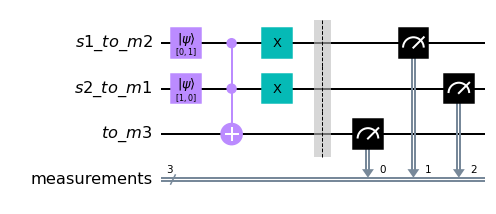
\includegraphics[width=0.85\linewidth]{./images/3qubit_qc.png}
	\caption{Circuit of the 3 Qubit Design}%
	\label{fig:3qubit_qc}%
\end{figure}

\textbf{Executing the circuits in both simulators and actual quantum computers:}
The codes are same as \hyperref[code:executing_the_quantum_circuit_on_a_simulator]{`Executing the Quantum Circuit on a Simulator'} and \hyperref[code:executing_the_quantum_circuit_on_a_quantum_computer]{`Executing the Quantum Circuit on an actual Quantum Computer'} section from the \hyperref[solution:1]{Approach 1}.

The result on the classical computer was exactly the same as the \hyperref[fig:5qubit_act]{previous result}. That on the Quantum Computer came out to be like \hyperref[fig:3qubit_act]{Figure 8}.

\begin{figure}[h]%
	\centering
	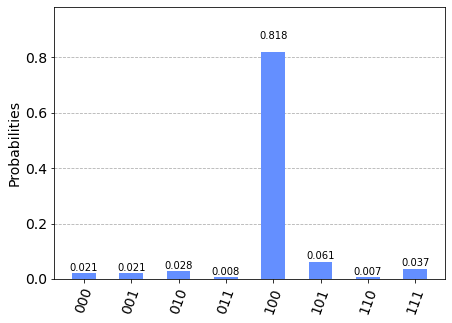
\includegraphics[width=0.85\linewidth]{./images/3qubit_act.png}
	\caption{\textbf{Histogram:} 3 Qubit Circuit executed on an actual Quantum Computer}%
	\label{fig:3qubit_act}%
\end{figure}